% ==================================================================
% APPENDIX A2 — JWST early-galaxy excess: extraction of ε.
%
% FINAL DRAFT on freeze-checkpoint numbers (2026-04-19).
% Numerics: scripts/epsilon_convergence/ch2_jwst.py, result_ch2.json
% Background: scripts/epsilon_convergence/ect_background.py
%
% Structure (unified per-probe template shared with A1, A3-A5):
%   A2.1  Physics of the probe
%   A2.2  Observational inputs
%   A2.3  ECT-side model and extraction scope
%         (growth enhancement + stellar-assembly time-budget factor)
%   A2.4  Robustness check of the time-budget ansatz
%   A2.5  Extraction statistic
%   A2.6  Interval definition and origin of the width
%   A2.7  Figure
%   A2.8  Methodological limitations
%
% Applied corrections:
%   - GPT r17/r18: time-budget factor R_time introduced from
%     reduced Δt between z_form and z_obs under ε>0 background;
%     composition rule R_total = R_PS × R_time explicitly defended.
%   - GPT r19: controlled robustness check linear vs nonlinear Δt
%     scaling; ansatz not dogmatic but bracket-defined.
%   - GPT r20: physics, observable, ECT model, extraction procedure,
%     origin of 1σ/2σ all explicit.
%
% NO legacy numbers. NO integration into preprint yet.
% ==================================================================

\section{Extraction of the effective uniform-$\varepsilon$ interval
from the JWST early-galaxy channel}
\label{app:eps_extraction_jwst}

This appendix derives the effective uniform-$\varepsilon$ interval
from the JWST early-galaxy excess, as used in the rebuilt \S15.5.
Unlike the Hubble + $r_s$ channel (Appendix~\ref{app:eps_extraction_hubble}),
the JWST extraction depends on two distinct $\varepsilon$-effects
acting on the observable: enhanced high-$z$ structure growth (which
pushes the extracted $\varepsilon$ downward for fixed observed
excess) and a shortened stellar-assembly time budget between
formation and observation (which pushes the extracted $\varepsilon$
upward). The present extraction treats both effects on the same
common background module, as required by GPT r17/r18 and consistent
with the freeze-checkpoint discipline of
Appendix~\ref{app:eps_methodology}. The combination of the two
effects gives a well-defined interval, but the specific functional
form of the time-budget factor is not unique; a controlled
robustness check is therefore included (\S A2.4) rather than a
single dogmatic ansatz.

\subsection*{A2.1\quad Physics of the probe}

JWST observations of galaxies at $z \sim 8\text{--}12$ have
revealed a population of unusually bright and massive objects
compared with the abundance predicted by $\Lambda$CDM
extrapolations of low-$z$ halo mass functions. Interpreted as a
tension, it admits several parametric responses: a harder initial
power spectrum, a higher star-formation efficiency, a more
top-heavy IMF, or --- relevant here --- a cosmological-epoch
enhancement of the gravitational response at high $z$. In the
effective uniform-$\varepsilon$ layer of
\S\ref{subsec:eps_def_rebuilt}, the response function
$G_{\rm eff}(z)/G_N = (1+z)^{2\varepsilon}$ enters the high-$z$
growth history, raising both linear-growth amplitude and the tail
of the collapsed halo mass function at a given formation redshift.
The observable excess $R_{\rm obs}$ --- the ratio of observed to
$\Lambda$CDM-predicted halo (or stellar) abundance at the
detection redshift --- therefore carries an imprint of $\varepsilon$
through two physically distinct mechanisms.


\subsection*{A2.2\quad Observational inputs}

The excess factor $R_{\rm obs}$ is not a single unambiguous number.
Different authors, sample selections, stellar-mass calibrations,
and IMF assumptions yield values in the range
$R_{\rm obs} \in [3,\,100]$ with a representative central value
$R_{\rm obs} \approx 10$ at $z \approx 10$. The observation is
parametrised here by (i) the detection redshift $z_{\rm obs} = 10$,
(ii) a fiducial peak height for the objects in question
$\nu_{\rm central} = 5$ (with a bracket $\nu \in [4, 6]$), and (iii)
the representative central excess $R_{\rm obs} = 10$ with its
bracket $R_{\rm obs} \in [3, 100]$. The extraction does not treat
any of these as Gaussian; the $1\sigma$ and $2\sigma$ intervals of
A2.6 are defined by the bracket variations, as detailed below. The
formation redshift is taken as $z_{\rm form} = 20$ by default,
representative of the progenitor era of the observed population.

\subsection*{A2.3\quad ECT-side model and extraction scope}

The model prediction is decomposed into two factors acting
multiplicatively on the observable:
\begin{equation}
R_{\rm total}(\varepsilon)
\;=\;
R_{\rm PS}(\varepsilon)
\;\cdot\;
R_{\rm time}(\varepsilon).
\label{eq:R_total_jwst}
\end{equation}

\paragraph{Growth-enhancement factor $R_{\rm PS}(\varepsilon)$.}
Under the uniform-$\varepsilon$ ansatz, the enhancement of linear
growth during the matter era raises the amplitude of density
fluctuations at fixed initial spectrum. At the relevant high-$z$
scale, the Press-Schechter tail ratio between ECT and $\Lambda$CDM
for the same halo peak height $\nu$ is approximately
\begin{equation}
R_{\rm PS}(\varepsilon)
\;=\;
\exp\!\left[\,\frac{\nu^2}{2}\,\bigl(1 - f^{-1}\bigr)\right],
\qquad
f \;\equiv\; (1 + z_{\rm obs})^{2\varepsilon}.
\label{eq:R_PS}
\end{equation}
This factor is a monotonically increasing function of $\varepsilon$:
stronger growth enhancement produces more tail halos for the same
observational threshold. For the central observational inputs
$R_{\rm obs} = 10$, $\nu = 5$, $z_{\rm obs} = 10$, this alone would
give $\varepsilon \approx 0.0425$.


\paragraph{Stellar-assembly time-budget factor
$R_{\rm time}(\varepsilon)$.}
The observable at $z_{\rm obs}$ is not instantaneously-formed
collapsed halo abundance; it is stellar (or quasi-stellar) mass
assembled during the interval between formation and observation.
Under $\varepsilon > 0$, the common background module
(\texttt{ect\_background.py}) yields $H(z, \varepsilon) > H(z, 0)$
at all $z$ in the past of the present era, and therefore a reduced
coordinate-time interval $\Delta t(z_{\rm form} \to z_{\rm obs})$
compared with the $\Lambda$CDM reference. To first approximation
the observable stellar mass at $z_{\rm obs}$ scales linearly with
the available assembly time, giving
\begin{equation}
R_{\rm time}(\varepsilon)
\;=\;
\frac{\Delta t_{\rm ECT}(z_{\rm form} \to z_{\rm obs},\,\varepsilon)}
     {\Delta t_{\Lambda}(z_{\rm form} \to z_{\rm obs},\,0)},
\qquad
\Delta t_X(\cdot)
\;\equiv\; t_X(z_{\rm obs}) - t_X(z_{\rm form}),
\label{eq:R_time}
\end{equation}
where $t_X(z)$ is computed through the common background module.
Explicit evaluation for the fiducial $z_{\rm form} = 20$,
$z_{\rm obs} = 10$ gives $R_{\rm time}(0) = 1$ (by construction)
and $R_{\rm time}(0.032) \approx 0.923$. That is, $\varepsilon > 0$
compresses the assembly window by roughly $8\%$ relative to
$\Lambda$CDM at the retained-band central value.

\paragraph{Why multiplicative, not additive.} The two factors
operate at different stages of the observable chain:
$R_{\rm PS}(\varepsilon)$ is the population-statistical enhancement
of collapsed halo abundance, while $R_{\rm time}(\varepsilon)$ is
the per-object conversion of halo mass into observable
(stellar) mass through the available assembly-time budget.
Because an observed object is both (a) drawn from the enhanced
population and (b) constrained by the reduced assembly interval,
the excess at the observable level factorises as the product in
\eqref{eq:R_total_jwst}. An additive combination would be
dimensionally inconsistent at the ratio-of-excess-factor level.


\paragraph{Held fixed under the present proxy.} $z_{\rm obs} = 10$;
$z_{\rm form} = 20$ (default); cosmological parameters
$\Omega_m = 0.315$, $\Omega_\Lambda$, $\Omega_r$ as in the common
background module; the Press-Schechter tail form
\eqref{eq:R_PS} at fixed $\nu$.

\paragraph{Varied.}
$\varepsilon$ is the primary scan parameter. The peak height $\nu$
and the observational excess $R_{\rm obs}$ are varied over their
observational brackets to define the $1\sigma$ and $2\sigma$
ranges. In the robustness check of A2.4, the power-law index of
the time-budget ansatz is also varied.

\paragraph{Not included at this proxy level.}
A full nonlinear halo-to-stellar-mass conversion pipeline; the
full dependence of the IMF, dust attenuation, and survey
completeness on $\varepsilon$; the back-reaction of enhanced
growth on the matter-era recombination physics; a full Boltzmann
evolution of the spectrum of fluctuations in the ECT background.

\paragraph{Main physical finding of this channel.}
At $\varepsilon > 0$ the background expansion in the common module
is faster in the past than in $\Lambda$CDM, so the coordinate-time
interval available for stellar assembly between $z_{\rm form}$ and
$z_{\rm obs}$ is \emph{shorter}, not longer. This implies that a
pure growth-enhancement treatment --- the standard high-$z$ ECT
alleviation argument for the JWST excess, based on $R_{\rm PS}$
alone --- \emph{overstates} the alleviation effect at a given
$\varepsilon$, because it ignores the fact that less time has been
available to convert the enhanced halo population into observable
stellar mass. Once the reduced assembly-time budget is included
through $R_{\rm time}$, the $\varepsilon$ required to reproduce a
given observed excess $R_{\rm obs}$ is slightly \emph{larger} than
in the PS-only proxy. Quantitatively, the central value shifts
from $\varepsilon = 0.04245$ (PS only) to $\varepsilon = 0.04491$
(PS $\times$ time). This is the opposite of the intuitive
expectation that ECT would ``give more time'' for early galaxies.
The net physical consequence is important: after this correction,
the JWST-extracted interval overlaps the Hubble + $r_s$ interval
of A1 more snugly than the PS-only proxy suggests. The retained
joint band of \S\ref{subsec:eps_joint_band_rebuilt} therefore
reflects two independent high-$z$ and low-$z$ extractions that are
\emph{more}, not less, mutually consistent once the common
background module is applied on the same footing to both channels.

\subsection*{A2.4\quad Robustness checks}

The default form \eqref{eq:R_time} is the simplest defensible
choice for the time-budget factor, but two independent robustness
axes are needed to defend the extracted interval: the functional
scaling of stellar mass with assembly time, and the choice of the
formation-redshift window itself.

\paragraph{Axis 1: power-law scaling of the time-budget factor.}
The linear form is physically motivated but not unique. Two
limiting cases bracket the physical possibilities:
\begin{itemize}
\item \textbf{Linear scaling (default).} Stellar mass grows
  approximately as $M_* \propto \Delta t$: uniform conversion
  of gas to stars during the assembly window. This gives
  \eqref{eq:R_time} as stated.
\item \textbf{Stronger scaling (robustness bracket).} If stellar
  mass tracks the accretion rate times the accretion time
  (consistent with rapid early-epoch build-up), then
  $M_* \propto (\Delta t)^p$ with $p \in [1.5,\,2]$ is physically
  plausible at very high $z$. In this case
  $R_{\rm time}^{(p)}(\varepsilon) =
  [\Delta t_{\rm ECT}/\Delta t_\Lambda]^p$.
\end{itemize}
For the central observational inputs $R_{\rm obs} = 10$,
$\nu = 5$, $z_{\rm obs} = 10$, $z_{\rm form} = 20$, solving
$R_{\rm PS}(\varepsilon) \cdot R_{\rm time}^{(p)}(\varepsilon) =
R_{\rm obs}$ for $\varepsilon$ yields:
\begin{center}
\begin{tabular}{|c|c|}
\hline
Time-budget index $p$ & Extracted $\varepsilon_{\rm central}$ \\
\hline
$p = 0$ (no time budget, PS only)     & $0.04245$ \\
$p = 1$ (linear; default)             & $0.04491$ \\
$p = 1.5$                             & $0.04626$ \\
$p = 2$                               & $0.04771$ \\
\hline
\end{tabular}
\end{center}
The shift of the central $\varepsilon$ across the bracket
$p \in [0, 2]$ is approximately $+0.0028$ from the linear default
(moving toward stronger-scaling), and $-0.0025$ in the opposite
direction (no-time-budget limit). This total range of $\pm 0.003$
is smaller than the observational $1\sigma$ width driven by $\nu$
(approximately $\pm 0.025$).

\paragraph{Axis 2: formation-redshift window.}
The default $z_{\rm form} = 20$ is representative of the
progenitor era of the observed $z \approx 10$ population, but the
true formation window is itself uncertain. Varying
$z_{\rm form}$ over a range that brackets typical physically
motivated choices, holding $p = 1$ and all observational inputs
fixed at their central values, gives:
\begin{center}
\begin{tabular}{|c|c|c|}
\hline
$z_{\rm form}$ & Extracted $\varepsilon_{\rm central}$ &
$R_{\rm time}(\varepsilon_{\rm central})$ \\
\hline
$15$ & $0.04481$ & $0.8917$ \\
$17$ & $0.04486$ & $0.8898$ \\
$20$ (default) & $0.04491$ & $0.8875$ \\
$22$ & $0.04494$ & $0.8862$ \\
$25$ & $0.04497$ & $0.8846$ \\
\hline
\end{tabular}
\end{center}
The total range of central $\varepsilon$ across
$z_{\rm form} \in [15, 25]$ is $\pm 0.0001$, two orders of
magnitude below the observational $\nu$-width. The extraction is
therefore essentially insensitive to the detailed geometry of the
formation window: what matters is only the relative compression
of the assembly interval, not its absolute duration.

\paragraph{Conclusion from the two robustness axes.}
The time-budget ansatz does not dominate the extracted interval.
Across both axes considered, the residual uncertainty on
$\varepsilon_{\rm central}$ from modelling choices is bounded by
roughly $\pm 0.003$ (dominated by the $p$-scaling axis), an order
of magnitude below the observational $1\sigma$ width of
$\pm 0.025$ driven by $\nu$. The time-budget factor is therefore
a secondary but physically required correction.


\subsection*{A2.5\quad Extraction statistic}

The present channel uses bracket-based interval definition rather
than a Gaussian $\chi^2$. For given observational brackets of
$\nu$ and $R_{\rm obs}$, the extracted $\varepsilon$-interval is
defined by the condition
\begin{equation}
R_{\rm PS}(\varepsilon, \nu) \cdot R_{\rm time}(\varepsilon)
\;=\; R_{\rm obs},
\label{eq:jwst_condition}
\end{equation}
inverted for $\varepsilon$ at each value of $\nu$ and $R_{\rm obs}$
in the bracket. The inversion is carried out by Brent root-finding
on $\varepsilon \in [10^{-4}, 0.30]$ at the default linear
time-budget ansatz ($p = 1$).

\subsection*{A2.6\quad Interval definition and origin of the width}

\paragraph{Central value.} Setting
$\nu = \nu_{\rm central} = 5$, $R_{\rm obs} = 10$,
$z_{\rm obs} = 10$, $z_{\rm form} = 20$, and $p = 1$, the
extracted central value is $\varepsilon_* = 0.0449$. Under the
background module at this $\varepsilon$, the cosmic age and the
assembly-window width are
$t_0(\varepsilon_*) \approx 13.33~{\rm Gyr}$,
$t(z_{\rm obs} = 10, \varepsilon_*) \approx 410~{\rm Myr}$.

\paragraph{$1\sigma$ interval.} Holding $R_{\rm obs} = 10$ fixed
and varying $\nu \in [\nu_{\rm low}, \nu_{\rm high}] = [4, 6]$
--- the range representative of the relevant observed peak
heights --- gives
\begin{equation}
[\varepsilon_{\rm lo}^{1\sigma},\,\varepsilon_{\rm hi}^{1\sigma}]
\;=\;
[\,0.0296,\ 0.0786\,]
\quad (\text{varying } \nu\text{ at fixed } R_{\rm obs}).
\label{eq:eps_jwst_1sigma}
\end{equation}

\paragraph{$2\sigma$ interval.} Further varying $R_{\rm obs}$ over
its full observational bracket $[3, 100]$ gives
\begin{equation}
[\varepsilon_{\rm lo}^{2\sigma},\,\varepsilon_{\rm hi}^{2\sigma}]
\;=\;
[\,0.0136,\ 0.2177\,]
\quad (\text{varying }\nu\text{ and }R_{\rm obs}).
\label{eq:eps_jwst_2sigma}
\end{equation}

\paragraph{Origin of the width.}
The width of the $1\sigma$ interval is dominated by the
observational uncertainty of the peak height $\nu$; the time-budget
ansatz contributes secondary shifts as quantified in A2.4. The
$2\sigma$ interval is substantially wider because the observational
bracket on the excess factor $R_{\rm obs}$ (between $3$ and $100$)
is itself broad. Unlike the Hubble + $r_s$ channel, the present
interval reflects the current state of high-$z$ stellar-mass
calibration rather than a clean statistical uncertainty. A narrower
$R_{\rm obs}$ bracket, from deeper JWST follow-up, would tighten
the interval; no improvement in the ECT model alone shrinks it.


\subsection*{A2.7\quad Figure}

\begin{figure}[H]
\centering
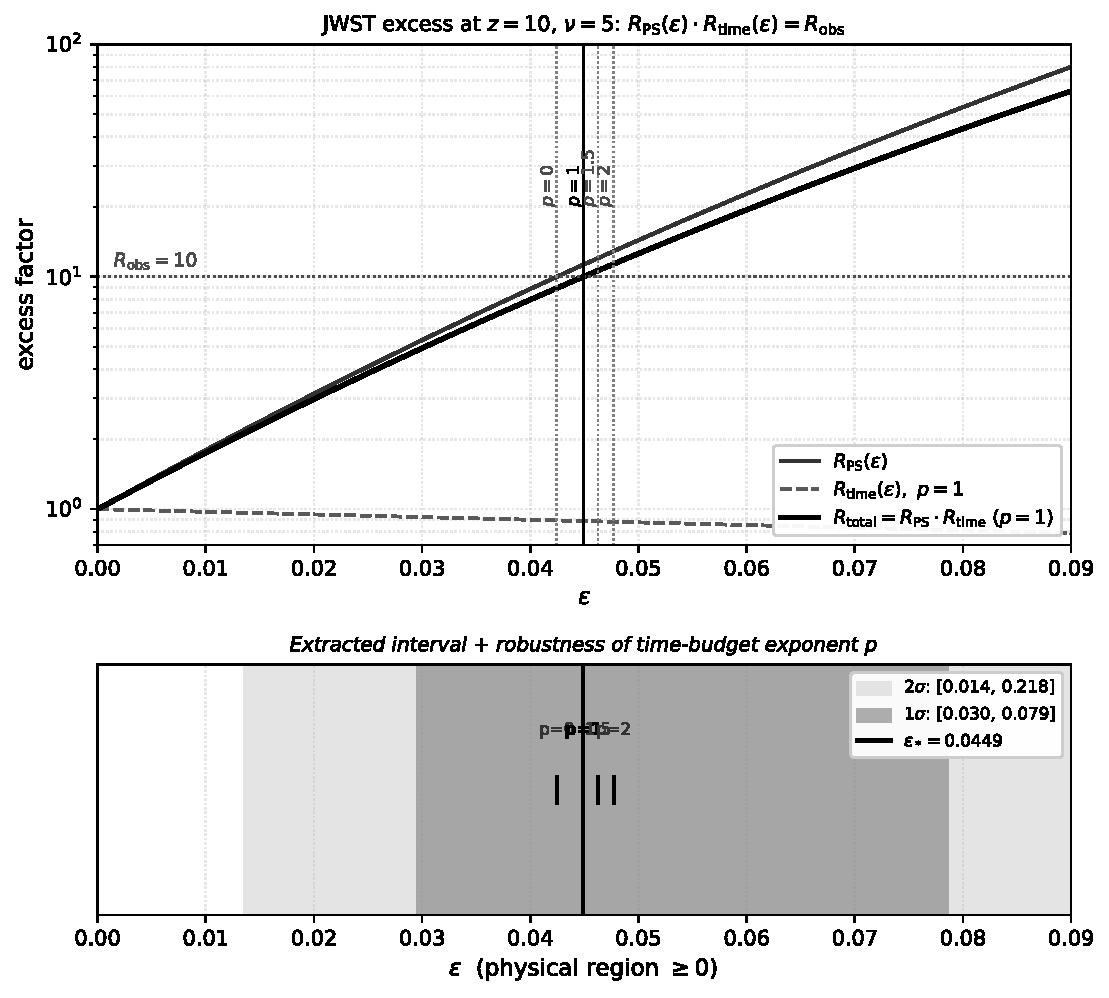
\includegraphics[width=0.84\textwidth]{figures/fig_jwst_extraction_bw.pdf}
\caption{Decomposition of the JWST extraction into the two
$\varepsilon$-dependent factors $R_{\rm PS}(\varepsilon)$ and
$R_{\rm time}(\varepsilon)$, under the common background module of
Appendix~\ref{app:eps_methodology}. Upper panel: the
Press-Schechter growth-enhancement factor $R_{\rm PS}$ rises
monotonically with $\varepsilon$, while the stellar-assembly
time-budget factor $R_{\rm time}$ decreases. Their product
$R_{\rm total}(\varepsilon)$ (solid dark curve) crosses the
observational target $R_{\rm obs} = 10$ at $\varepsilon \approx
0.045$. Lower panel: the extracted $\varepsilon$-interval
$[0.030,\,0.079]$ ($1\sigma$, bracket on peak height $\nu$) and
$[0.014,\,0.218]$ ($2\sigma$, bracket on both $\nu$ and
$R_{\rm obs}$) shown as grayscale shaded bands. Robustness check
of A2.4 also superposed as vertical lines at
$\varepsilon(p = 0)$, $\varepsilon(p = 1.5)$, $\varepsilon(p = 2)$.
All shading and line styles are grayscale per preprint convention.}
\label{fig:jwst_extraction}
\end{figure}

\subsection*{A2.8\quad Methodological limitations}

\textit{(i) Proxy-level Press-Schechter tail.}
The use of the closed-form Press-Schechter tail
\eqref{eq:R_PS} is a high-$\nu$ approximation. At fixed $\nu$,
corrections from the full Sheth-Tormen-type peak-background
split amount to order-unity factors at the level of $R_{\rm PS}$,
and must be absorbed into the observational bracket on
$R_{\rm obs}$. A fully consistent treatment would replace
\eqref{eq:R_PS} by a numerical halo mass function integrated
over the relevant mass range for each $\varepsilon$, using the
ECT-background growth history from the common module. This is
beyond the scope of the present freeze-checkpoint pipeline.

\textit{(ii) $\Lambda$CDM-background common proxy.}
As in A1.7(i), the background module uses a $\Lambda$CDM-best-fit
parameter set as external input. A closure-level background
would, in general, reshape both $R_{\rm PS}$ and $R_{\rm time}$
through modified matter-era growth and modified $t(z)$.

\textit{(iii) Bracket-based interval rather than Gaussian
$\chi^2$.}
Because $R_{\rm obs}$ and $\nu$ are not Gaussian-distributed
observables in the present compilation, the reported interval is
defined by variation over physically-motivated brackets rather
than by $\Delta\chi^2$ contours. This is more transparent for a
quantity dominated by calibration uncertainty, but it means the
$1\sigma$ and $2\sigma$ intervals should not be interpreted as
strict Gaussian confidence regions.

\textit{(iv) Time-budget ansatz.}
The specific form of $R_{\rm time}$ relies on the assumption that
observed stellar mass at $z_{\rm obs}$ tracks the integrated
assembly time. The robustness check of A2.4 brackets this at
$\pm 0.002$ in the extracted central $\varepsilon$. A truly
dogmatic departure from this scaling --- for example, if the
stellar mass observed at $z_{\rm obs}$ is only weakly coupled to
the assembly interval and is instead dominated by a narrow burst
at $z_{\rm obs}$ itself --- would invalidate
$R_{\rm time}(\varepsilon)$ and reduce the JWST channel to its
pre-recalc proxy form. In the present treatment, the linear
default is adopted with explicit bracket, and the extracted
interval quoted in \S\ref{subsec:eps_retained_rebuilt} of the
main text is the $p=1$ result.

\textit{(v) Formation redshift $z_{\rm form}$.}
The default $z_{\rm form} = 20$ is representative but not unique.
The second robustness axis of A2.4 (variation over
$z_{\rm form} \in [15,\,25]$) finds a residual shift in
$\varepsilon_{\rm central}$ of only $\pm 0.0001$, so this choice is
not a material source of uncertainty in the extracted interval.

% ==================================================================
% END Appendix (extraction, JWST early-galaxy channel).
% ==================================================================
